
%% bare_jrnl_compsoc.tex
%% V1.4b
%% 2015/08/26
%% by Michael Shell
%% See:
%% http://www.michaelshell.org/
%% for current contact information.
%%
%% This is a skeleton file demonstrating the use of IEEEtran.cls
%% (requires IEEEtran.cls version 1.8b or later) with an IEEE
%% Computer Society journal paper.
%%
%% Support sites:
%% http://www.michaelshell.org/tex/ieeetran/
%% http://www.ctan.org/pkg/ieeetran
%% and
%% http://www.ieee.org/

%%*************************************************************************
%% Legal Notice:
%% This code is offered as-is without any warranty either expressed or
%% implied; without even the implied warranty of MERCHANTABILITY or
%% FITNESS FOR A PARTICULAR PURPOSE! 
%% User assumes all risk.
%% In no event shall the IEEE or any contributor to this code be liable for
%% any damages or losses, including, but not limited to, incidental,
%% consequential, or any other damages, resulting from the use or misuse
%% of any information contained here.
%%
%% All comments are the opinions of their respective authors and are not
%% necessarily endorsed by the IEEE.
%%
%% This work is distributed under the LaTeX Project Public License (LPPL)
%% ( http://www.latex-project.org/ ) version 1.3, and may be freely used,
%% distributed and modified. A copy of the LPPL, version 1.3, is included
%% in the base LaTeX documentation of all distributions of LaTeX released
%% 2003/12/01 or later.
%% Retain all contribution notices and credits.
%% ** Modified files should be clearly indicated as such, including  **
%% ** renaming them and changing author support contact information. **
%%*************************************************************************


% *** Authors should verify (and, if needed, correct) their LaTeX system  ***
% *** with the testflow diagnostic prior to trusting their LaTeX platform ***
% *** with production work. The IEEE's font choices and paper sizes can   ***
% *** trigger bugs that do not appear when using other class files.       ***                          ***
% The testflow support page is at:
% http://www.michaelshell.org/tex/testflow/


\documentclass[10pt,journal,compsoc]{IEEEtran}
%
% If IEEEtran.cls has not been installed into the LaTeX system files,
% manually specify the path to it like:
% \documentclass[10pt,journal,compsoc]{../sty/IEEEtran}





% Some very useful LaTeX packages include:
% (uncomment the ones you want to load)


% *** MISC UTILITY PACKAGES ***
%
%\usepackage{ifpdf}
% Heiko Oberdiek's ifpdf.sty is very useful if you need conditional
% compilation based on whether the output is pdf or dvi.
% usage:
% \ifpdf
%   % pdf code
% \else
%   % dvi code
% \fi
% The latest version of ifpdf.sty can be obtained from:
% http://www.ctan.org/pkg/ifpdf
% Also, note that IEEEtran.cls V1.7 and later provides a builtin
% \ifCLASSINFOpdf conditional that works the same way.
% When switching from latex to pdflatex and vice-versa, the compiler may
% have to be run twice to clear warning/error messages.






% *** CITATION PACKAGES ***
%
\ifCLASSOPTIONcompsoc
  % IEEE Computer Society needs nocompress option
  % requires cite.sty v4.0 or later (November 2003)
  \usepackage[nocompress]{cite}
\else
  % normal IEEE
  \usepackage{cite}
\fi
% cite.sty was written by Donald Arseneau
% V1.6 and later of IEEEtran pre-defines the format of the cite.sty package
% \cite{} output to follow that of the IEEE. Loading the cite package will
% result in citation numbers being automatically sorted and properly
% "compressed/ranged". e.g., [1], [9], [2], [7], [5], [6] without using
% cite.sty will become [1], [2], [5]--[7], [9] using cite.sty. cite.sty's
% \cite will automatically add leading space, if needed. Use cite.sty's
% noadjust option (cite.sty V3.8 and later) if you want to turn this off
% such as if a citation ever needs to be enclosed in parenthesis.
% cite.sty is already installed on most LaTeX systems. Be sure and use
% version 5.0 (2009-03-20) and later if using hyperref.sty.
% The latest version can be obtained at:
% http://www.ctan.org/pkg/cite
% The documentation is contained in the cite.sty file itself.
%
% Note that some packages require special options to format as the Computer
% Society requires. In particular, Computer Society  papers do not use
% compressed citation ranges as is done in typical IEEE papers
% (e.g., [1]-[4]). Instead, they list every citation separately in order
% (e.g., [1], [2], [3], [4]). To get the latter we need to load the cite
% package with the nocompress option which is supported by cite.sty v4.0
% and later. Note also the use of a CLASSOPTION conditional provided by
% IEEEtran.cls V1.7 and later.





% *** GRAPHICS RELATED PACKAGES ***
%
\ifCLASSINFOpdf
  % \usepackage[pdftex]{graphicx}
  % declare the path(s) where your graphic files are
  % \graphicspath{{../pdf/}{../jpeg/}}
  % and their extensions so you won't have to specify these with
  % every instance of \includegraphics
  % \DeclareGraphicsExtensions{.pdf,.jpeg,.png}
\else
  % or other class option (dvipsone, dvipdf, if not using dvips). graphicx
  % will default to the driver specified in the system graphics.cfg if no
  % driver is specified.
  % \usepackage[dvips]{graphicx}
  % declare the path(s) where your graphic files are
  % \graphicspath{{../eps/}}
  % and their extensions so you won't have to specify these with
  % every instance of \includegraphics
  % \DeclareGraphicsExtensions{.eps}
\fi
% graphicx was written by David Carlisle and Sebastian Rahtz. It is
% required if you want graphics, photos, etc. graphicx.sty is already
% installed on most LaTeX systems. The latest version and documentation
% can be obtained at: 
% http://www.ctan.org/pkg/graphicx
% Another good source of documentation is "Using Imported Graphics in
% LaTeX2e" by Keith Reckdahl which can be found at:
% http://www.ctan.org/pkg/epslatex
%
% latex, and pdflatex in dvi mode, support graphics in encapsulated
% postscript (.eps) format. pdflatex in pdf mode supports graphics
% in .pdf, .jpeg, .png and .mps (metapost) formats. Users should ensure
% that all non-photo figures use a vector format (.eps, .pdf, .mps) and
% not a bitmapped formats (.jpeg, .png). The IEEE frowns on bitmapped formats
% which can result in "jaggedy"/blurry rendering of lines and letters as
% well as large increases in file sizes.
%
% You can find documentation about the pdfTeX application at:
% http://www.tug.org/applications/pdftex






% *** MATH PACKAGES ***
%
%\usepackage{amsmath}
% A popular package from the American Mathematical Society that provides
% many useful and powerful commands for dealing with mathematics.
%
% Note that the amsmath package sets \interdisplaylinepenalty to 10000
% thus preventing page breaks from occurring within multiline equations. Use:
%\interdisplaylinepenalty=2500
% after loading amsmath to restore such page breaks as IEEEtran.cls normally
% does. amsmath.sty is already installed on most LaTeX systems. The latest
% version and documentation can be obtained at:
% http://www.ctan.org/pkg/amsmath





% *** SPECIALIZED LIST PACKAGES ***
%
%\usepackage{algorithmic}
% algorithmic.sty was written by Peter Williams and Rogerio Brito.
% This package provides an algorithmic environment fo describing algorithms.
% You can use the algorithmic environment in-text or within a figure
% environment to provide for a floating algorithm. Do NOT use the algorithm
% floating environment provided by algorithm.sty (by the same authors) or
% algorithm2e.sty (by Christophe Fiorio) as the IEEE does not use dedicated
% algorithm float types and packages that provide these will not provide
% correct IEEE style captions. The latest version and documentation of
% algorithmic.sty can be obtained at:
% http://www.ctan.org/pkg/algorithms
% Also of interest may be the (relatively newer and more customizable)
% algorithmicx.sty package by Szasz Janos:
% http://www.ctan.org/pkg/algorithmicx




% *** ALIGNMENT PACKAGES ***
%
%\usepackage{array}
% Frank Mittelbach's and David Carlisle's array.sty patches and improves
% the standard LaTeX2e array and tabular environments to provide better
% appearance and additional user controls. As the default LaTeX2e table
% generation code is lacking to the point of almost being broken with
% respect to the quality of the end results, all users are strongly
% advised to use an enhanced (at the very least that provided by array.sty)
% set of table tools. array.sty is already installed on most systems. The
% latest version and documentation can be obtained at:
% http://www.ctan.org/pkg/array


% IEEEtran contains the IEEEeqnarray family of commands that can be used to
% generate multiline equations as well as matrices, tables, etc., of high
% quality.




% *** SUBFIGURE PACKAGES ***
%\ifCLASSOPTIONcompsoc
%  \usepackage[caption=false,font=footnotesize,labelfont=sf,textfont=sf]{subfig}
%\else
%  \usepackage[caption=false,font=footnotesize]{subfig}
%\fi
% subfig.sty, written by Steven Douglas Cochran, is the modern replacement
% for subfigure.sty, the latter of which is no longer maintained and is
% incompatible with some LaTeX packages including fixltx2e. However,
% subfig.sty requires and automatically loads Axel Sommerfeldt's caption.sty
% which will override IEEEtran.cls' handling of captions and this will result
% in non-IEEE style figure/table captions. To prevent this problem, be sure
% and invoke subfig.sty's "caption=false" package option (available since
% subfig.sty version 1.3, 2005/06/28) as this is will preserve IEEEtran.cls
% handling of captions.
% Note that the Computer Society format requires a sans serif font rather
% than the serif font used in traditional IEEE formatting and thus the need
% to invoke different subfig.sty package options depending on whether
% compsoc mode has been enabled.
%
% The latest version and documentation of subfig.sty can be obtained at:
% http://www.ctan.org/pkg/subfig




% *** FLOAT PACKAGES ***
%
%\usepackage{fixltx2e}
% fixltx2e, the successor to the earlier fix2col.sty, was written by
% Frank Mittelbach and David Carlisle. This package corrects a few problems
% in the LaTeX2e kernel, the most notable of which is that in current
% LaTeX2e releases, the ordering of single and double column floats is not
% guaranteed to be preserved. Thus, an unpatched LaTeX2e can allow a
% single column figure to be placed prior to an earlier double column
% figure.
% Be aware that LaTeX2e kernels dated 2015 and later have fixltx2e.sty's
% corrections already built into the system in which case a warning will
% be issued if an attempt is made to load fixltx2e.sty as it is no longer
% needed.
% The latest version and documentation can be found at:
% http://www.ctan.org/pkg/fixltx2e


%\usepackage{stfloats}
% stfloats.sty was written by Sigitas Tolusis. This package gives LaTeX2e
% the ability to do double column floats at the bottom of the page as well
% as the top. (e.g., "\begin{figure*}[!b]" is not normally possible in
% LaTeX2e). It also provides a command:
%\fnbelowfloat
% to enable the placement of footnotes below bottom floats (the standard
% LaTeX2e kernel puts them above bottom floats). This is an invasive package
% which rewrites many portions of the LaTeX2e float routines. It may not work
% with other packages that modify the LaTeX2e float routines. The latest
% version and documentation can be obtained at:
% http://www.ctan.org/pkg/stfloats
% Do not use the stfloats baselinefloat ability as the IEEE does not allow
% \baselineskip to stretch. Authors submitting work to the IEEE should note
% that the IEEE rarely uses double column equations and that authors should try
% to avoid such use. Do not be tempted to use the cuted.sty or midfloat.sty
% packages (also by Sigitas Tolusis) as the IEEE does not format its papers in
% such ways.
% Do not attempt to use stfloats with fixltx2e as they are incompatible.
% Instead, use Morten Hogholm'a dblfloatfix which combines the features
% of both fixltx2e and stfloats:
%
% \usepackage{dblfloatfix}
% The latest version can be found at:
% http://www.ctan.org/pkg/dblfloatfix




%\ifCLASSOPTIONcaptionsoff
%  \usepackage[nomarkers]{endfloat}
% \let\MYoriglatexcaption\caption
% \renewcommand{\caption}[2][\relax]{\MYoriglatexcaption[#2]{#2}}
%\fi
% endfloat.sty was written by James Darrell McCauley, Jeff Goldberg and 
% Axel Sommerfeldt. This package may be useful when used in conjunction with 
% IEEEtran.cls'  captionsoff option. Some IEEE journals/societies require that
% submissions have lists of figures/tables at the end of the paper and that
% figures/tables without any captions are placed on a page by themselves at
% the end of the document. If needed, the draftcls IEEEtran class option or
% \CLASSINPUTbaselinestretch interface can be used to increase the line
% spacing as well. Be sure and use the nomarkers option of endfloat to
% prevent endfloat from "marking" where the figures would have been placed
% in the text. The two hack lines of code above are a slight modification of
% that suggested by in the endfloat docs (section 8.4.1) to ensure that
% the full captions always appear in the list of figures/tables - even if
% the user used the short optional argument of \caption[]{}.
% IEEE papers do not typically make use of \caption[]'s optional argument,
% so this should not be an issue. A similar trick can be used to disable
% captions of packages such as subfig.sty that lack options to turn off
% the subcaptions:
% For subfig.sty:
% \let\MYorigsubfloat\subfloat
% \renewcommand{\subfloat}[2][\relax]{\MYorigsubfloat[]{#2}}
% However, the above trick will not work if both optional arguments of
% the \subfloat command are used. Furthermore, there needs to be a
% description of each subfigure *somewhere* and endfloat does not add
% subfigure captions to its list of figures. Thus, the best approach is to
% avoid the use of subfigure captions (many IEEE journals avoid them anyway)
% and instead reference/explain all the subfigures within the main caption.
% The latest version of endfloat.sty and its documentation can obtained at:
% http://www.ctan.org/pkg/endfloat
%
% The IEEEtran \ifCLASSOPTIONcaptionsoff conditional can also be used
% later in the document, say, to conditionally put the References on a 
% page by themselves.




% *** PDF, URL AND HYPERLINK PACKAGES ***
%
%\usepackage{url}
% url.sty was written by Donald Arseneau. It provides better support for
% handling and breaking URLs. url.sty is already installed on most LaTeX
% systems. The latest version and documentation can be obtained at:
% http://www.ctan.org/pkg/url
% Basically, \url{my_url_here}.

\usepackage[utf8]{inputenc} % allow utf-8 input
\usepackage[T1]{fontenc}    % use 8-bit T1 fonts
%\usepackage{hyperref}       % hyperlinks
\usepackage[hidelinks]{hyperref}
\usepackage{url}            % simple URL typesetting
\usepackage{booktabs}       % professional-quality tables
\usepackage{amsfonts}       % blackboard math symbols
\usepackage{nicefrac}       % compact symbols for 1/2, etc.
\usepackage{microtype}      % microtypography
\usepackage{amsmath}
\usepackage{subcaption}
\usepackage{graphicx}
%\usepackage{makecell}
%\usepackage{subfigure}

\newenvironment{mycell}[1]
{
	\begin{minipage}{#1}
		\begin{center}
			\vspace*{0.15cm}
		}
		{
			\vspace*{0.1cm}
		\end{center}
	\end{minipage}
}




% *** Do not adjust lengths that control margins, column widths, etc. ***
% *** Do not use packages that alter fonts (such as pslatex).         ***
% There should be no need to do such things with IEEEtran.cls V1.6 and later.
% (Unless specifically asked to do so by the journal or conference you plan
% to submit to, of course. )


% correct bad hyphenation here
\hyphenation{op-tical net-works semi-conduc-tor}


\begin{document}
%
% paper title
% Titles are generally capitalized except for words such as a, an, and, as,
% at, but, by, for, in, nor, of, on, or, the, to and up, which are usually
% not capitalized unless they are the first or last word of the title.
% Linebreaks \\ can be used within to get better formatting as desired.
% Do not put math or special symbols in the title.
\title{Generalised Off-line Training of Deep\\Spiking Neural Networks}
%
%
% author names and IEEE memberships
% note positions of commas and nonbreaking spaces ( ~ ) LaTeX will not break
% a structure at a ~ so this keeps an author's name from being broken across
% two lines.
% use \thanks{} to gain access to the first footnote area
% a separate \thanks must be used for each paragraph as LaTeX2e's \thanks
% was not built to handle multiple paragraphs
%
%
%\IEEEcompsocitemizethanks is a special \thanks that produces the bulleted
% lists the Computer Society journals use for "first footnote" author
% affiliations. Use \IEEEcompsocthanksitem which works much like \item
% for each affiliation group. When not in compsoc mode,
% \IEEEcompsocitemizethanks becomes like \thanks and
% \IEEEcompsocthanksitem becomes a line break with idention. This
% facilitates dual compilation, although admittedly the differences in the
% desired content of \author between the different types of papers makes a
% one-size-fits-all approach a daunting prospect. For instance, compsoc 
% journal papers have the author affiliations above the "Manuscript
% received ..."  text while in non-compsoc journals this is reversed. Sigh.

\author{Qian~Liu, Yunhua~Chen, Garibaldi~Pineda-Garc\'ia, and~Steve~Furber,~\IEEEmembership{Member,~IEEE,}% <-this % stops a space
\IEEEcompsocitemizethanks{\IEEEcompsocthanksitem Qian~Liu, Garibaldi~Pineda-Garc\'ia\, and Steve Furber are with the School of Computer Science, The University of Manchester, Manchester, UK, M13 9PL.\protect\\
% note need leading \protect in front of \\ to get a newline within \thanks as
% \\ is fragile and will error, could use \hfil\break instead.
E-mail: \{qian.liu-3, garibaldi.pinedagarcia, steve.furber\}@manchester.ac.uk
\IEEEcompsocthanksitem Yunhua Chen is with the School of Computer Science, Guangdong University of Technology, Guangzhou, China.\protect\\
E-mail: yhchen@gdut.edu.cn}% <-this % stops an unwanted space
%\thanks{Manuscript received April 19, 2005; revised August 26, 2015.}
}

% note the % following the last \IEEEmembership and also \thanks - 
% these prevent an unwanted space from occurring between the last author name
% and the end of the author line. i.e., if you had this:
% 
% \author{....lastname \thanks{...} \thanks{...} }
%                     ^------------^------------^----Do not want these spaces!
%
% a space would be appended to the last name and could cause every name on that
% line to be shifted left slightly. This is one of those "LaTeX things". For
% instance, "\textbf{A} \textbf{B}" will typeset as "A B" not "AB". To get
% "AB" then you have to do: "\textbf{A}\textbf{B}"
% \thanks is no different in this regard, so shield the last } of each \thanks
% that ends a line with a % and do not let a space in before the next \thanks.
% Spaces after \IEEEmembership other than the last one are OK (and needed) as
% you are supposed to have spaces between the names. For what it is worth,
% this is a minor point as most people would not even notice if the said evil
% space somehow managed to creep in.



% The paper headers
%\markboth{Journal of \LaTeX\ Class Files,~Vol.~14, No.~8, August~2015}%
%{Shell \MakeLowercase{\textit{et al.}}: Bare Demo of IEEEtran.cls for Computer Society Journals}
% The only time the second header will appear is for the odd numbered pages
% after the title page when using the twoside option.
% 
% *** Note that you probably will NOT want to include the author's ***
% *** name in the headers of peer review papers.                   ***
% You can use \ifCLASSOPTIONpeerreview for conditional compilation here if
% you desire.



% The publisher's ID mark at the bottom of the page is less important with
% Computer Society journal papers as those publications place the marks
% outside of the main text columns and, therefore, unlike regular IEEE
% journals, the available text space is not reduced by their presence.
% If you want to put a publisher's ID mark on the page you can do it like
% this:
%\IEEEpubid{0000--0000/00\$00.00~\copyright~2015 IEEE}
% or like this to get the Computer Society new two part style.
%\IEEEpubid{\makebox[\columnwidth]{\hfill 0000--0000/00/\$00.00~\copyright~2015 IEEE}%
%\hspace{\columnsep}\makebox[\columnwidth]{Published by the IEEE Computer Society\hfill}}
% Remember, if you use this you must call \IEEEpubidadjcol in the second
% column for its text to clear the IEEEpubid mark (Computer Society jorunal
% papers don't need this extra clearance.)



% use for special paper notices
%\IEEEspecialpapernotice{(Invited Paper)}



% for Computer Society papers, we must declare the abstract and index terms
% PRIOR to the title within the \IEEEtitleabstractindextext IEEEtran
% command as these need to go into the title area created by \maketitle.
% As a general rule, do not put math, special symbols or citations
% in the abstract or keywords.
\IEEEtitleabstractindextext{%
\begin{abstract}
Spiking neural networks~(SNNs) can be trained by first training an equivalent ANN and then transferring the trained weights to the SNN, but there are two significant problems to be solved.
First, an accurate activation function is needed to model the neural dynamics of spiking neurons, and the previously proposed activation function, Noisy Softplus~(NSP), has shown to be a good match to the response activity of Leaky Integrate-and-Fire~(LIF) neurons.
The second problem is mapping the abstract numerical values of the ANN to concrete physical units in the SNN, such as current and firing rate.
In this paper, we introduce the parametric activation function~[PAF; $y = p \times f(x)$], to tackle the second problem.
With these problems solved, SNN training can be simplified as: (1) estimate parameter $p$ for PAF according to biological configurations of LIF neurons, and (2) use PAF instead of conventional activation functions to train an equivalent ANN.
The trained weights can be transferred directly into the spiking version of the same network without further conversion.
In addition, we propose a fine tuning method as an option which helps the trained network to closer match the SNN.
Based on this generalised training method, we achieve the best SNN accuracy on the MNIST task using LIF neurons, 98.85\%, on a 6-layer spiking convolutional neural network~(ConvNet).

\end{abstract}

% Note that keywords are not normally used for peerreview papers.
\begin{IEEEkeywords}
Spiking Neural Networks, Deep Learning, training, Convolutional Neural Networks, activation function.
\end{IEEEkeywords}}


% make the title area
\maketitle


% To allow for easy dual compilation without having to reenter the
% abstract/keywords data, the \IEEEtitleabstractindextext text will
% not be used in maketitle, but will appear (i.e., to be "transported")
% here as \IEEEdisplaynontitleabstractindextext when the compsoc 
% or transmag modes are not selected <OR> if conference mode is selected 
% - because all conference papers position the abstract like regular
% papers do.
\IEEEdisplaynontitleabstractindextext
% \IEEEdisplaynontitleabstractindextext has no effect when using
% compsoc or transmag under a non-conference mode.



% For peer review papers, you can put extra information on the cover
% page as needed:
% \ifCLASSOPTIONpeerreview
% \begin{center} \bfseries EDICS Category: 3-BBND \end{center}
% \fi
%
% For peerreview papers, this IEEEtran command inserts a page break and
% creates the second title. It will be ignored for other modes.
\IEEEpeerreviewmaketitle



\IEEEraisesectionheading{\section{Introduction}\label{sec:introduction}}
% Computer Society journal (but not conference!) papers do something unusual
% with the very first section heading (almost always called "Introduction").
% They place it ABOVE the main text! IEEEtran.cls does not automatically do
% this for you, but you can achieve this effect with the provided
% \IEEEraisesectionheading{} command. Note the need to keep any \label that
% is to refer to the section immediately after \section in the above as
% \IEEEraisesectionheading puts \section within a raised box.




% The very first letter is a 2 line initial drop letter followed
% by the rest of the first word in caps (small caps for compsoc).
% 
% form to use if the first word consists of a single letter:
% \IEEEPARstart{A}{demo} file is ....
% 
% form to use if you need the single drop letter followed by
% normal text (unknown if ever used by the IEEE):
% \IEEEPARstart{A}{}demo file is ....
% 
% Some journals put the first two words in caps:
% \IEEEPARstart{T}{his demo} file is ....
% 
% Here we have the typical use of a "T" for an initial drop letter
% and "HIS" in caps to complete the first word.
\IEEEPARstart{A}{dvances} in computing power and machine learning have endowed computers with rapidly growing performance in cognitive tasks such as recognising objects~\cite{deng2009imagenet} and playing GO~\cite{silver2016mastering};
these tasks were once dominated by human intelligence and solved by biological neurons in the brain.
However, humans and many other animals still outperform computers in practical tasks, such as vision, and in terms of size and energy cost by several orders of magnitude.
For instance, AlphaGO~\cite{silver2016mastering} has a power consumption of 1~MW on its $1,920$ CPUs and 280 GPUs when playing the game with one of the best human players whose brain is rated at 20~W~\cite{drubach2000brain}.
Although we are still far from understanding the brain thoroughly, it is believed that the performance gap between computation in the biological nervous system and in a computer lies in the nature of the fundamental computing units and how they compute.
Typical computers employ Boolean logic and deterministic digital operations usually based on synchronous clocks while nervous systems employ parallel, distributed, event-driven, stochastically unreliable components~\cite{indiveri2009artificial}: neurons.
These impressive disparities in cognitive capabilities and energy consumption drive research into biologically-plausible spiking neurons and brain inspired computers, known as Neuromorphic Engineering~(NE).
%Today	we	stand	poised	on	the	brink	of	a	new	era	of	compu:ng	in	which	technology	is	more	
%consumable,	insight-driven	and	cogni:ve.	IBM	Research	is	exploring	and	developing	the	
%enabling	technologies	that	will	transform	the	way	computers	are	used	
%Ginni	Rome]y	
%IBM	President,	Chairman	and	CEO	




%Two aims
NE was proposed by Carver Mead in the late 1980s \cite{Mead:1989:AVN:64998} to build analogue circuits which mimic biological neural cells and the architecture of the nervous system using Very-Large-Scale Integration (VLSI) technology.
With the ultimate goal of equipping neuromorphic machines with genuine intelligence, 
%~\cite{konar1999artificial}, also known as `Neuromorphic Cognition'~\cite{indiveri2009artificial},
the objectives of NE can be summarised as follows~\cite{furber2007neural}:
\begin{itemize}
	\item brain modelling: for neuroscientists to understand the brain by modelling and simulating the activities of biological neurons; 
	\item neuromorphic computing: for engineers to build brain-like machines by applying biological principles to computers.
\end{itemize}
The aims complement each other; building a biologically inspired computer requires a better understanding of the brain, and simulating brain activities at large scale and in real time is feasible only on massively-parallel neuromorphic hardware.



%Since around 2004 to 2005, `Dennard's Law' has no longer been followed~\cite{bohr200730}, so as transistors get smaller their power density no longer stays constant but starts to increase.
%The breakdown of Dennard scaling and the problem of power dissipation drove chip manufacturers to multi/many-core architecture.
%However, the increased number of active transistors in a multi-core chip costs more power consumption thus creating the prospect that some fraction of the cores will have to remain completely powered-off given the thermal design power constraint.
%Dark silicon~\cite{esmaeilzadeh2011dark} addresses the issue of inactive areas of a multi-core chip, which could be 50\% of nodes in an 8~nm technology.
%Neuromorphic engineering offers a potential solution for power dissipation by applying the biological features of event-driven, hybrid analogue/digital, unreliable components to computers.
%Moreover, most of the neural interconnections in the brain are local, and the `memory' units attach to the `computation' node in a neuron.
%Therefore, learning from biology may give computers an alternative to the conventional Von Neumann architecture and thus may solve the problem of the microprocessor/memory performance gap~\cite{wulf1995hitting}, also known as the Von Neumann bottleneck, where the system speed is determined and limited by the memory performance.

%Why SNN
Spiking Neural Networks (SNNs), comprised of spiking neurons, hold the key to address the dual aims of understanding brain functions and building brain-like machines.
The spiking neuron mathematically models the dynamics of a single neuron with biological realism and the network describes the architecture of the neural connections and the information transmission among them; readers can refer to Chapter~\ref{cha:bkg} for more detail.
Therefore, neuroscientists are able to reproduce the recorded neural dynamics and activities from \textit{in-vivo/vitro} experiments to verify their models and measure the progress of brain understanding,
while computer engineers can focus on the hardware implementations of the spiking neurons and the interconnections between them to build energy-efficient neuromorphic hardware.

Over the last decade, considerable development has taken place in NE where simulations of massive SNNs~\cite{markram2006blue,ananthanarayanan2009cat} have proved to be significantly useful in understanding the brain, and large-scale neuromorphic platforms have been launched to simulate SNNs in hardware.
%, such as the High Input Count Analog Neural Network (HI-CANN)~\cite{schemmel2010wafer}, Neurogrid~\cite{benjamin2014neurogrid}, SpiNNaker~\cite{furber2014spinnaker}, TrueNorth~\cite{merolla2014million}, and HiAER-IFAT~\cite{yu201265k}.
These neuromorphic computers develop into energy-efficient systems by implementing neurons, synapses and neuronal communications on analogue circuits~\cite{schemmel2010wafer,benjamin2014neurogrid,yu201265k} or exploiting parallel low-power microprocessors on digital hardware~\cite{furber2014spinnaker,merolla2014million}. 
%Some of these neuromorphic computers~\cite{schemmel2010wafer,benjamin2014neurogrid,merolla2014million} use non-Von Neumann architectures to mimic the characteristics of parallelism, scalability, and fault-tolerance of the neural system.
%Instead of executing sequential instructions and building systems of separated computing and memory units, they rather copy the nature of the brain; implementing neurons, synapses and neuronal communications on analogue/digital microelectronics.
%Therefore this novel architecture may solve the problem of the microprocessor/memory performance gap~\cite{wulf1995hitting}, also known as the Von Neumann bottleneck, where the system speed is determined and limited by the memory performance;
%and at the same time, these neuromorphic computers develop into energy-efficient systems by reducing the energy used for data movement between processors and memories, and by employing event-based computing. 
Thus, the neuromorphic hardware systems composed with those have successfully demonstrated decreased energy cost of SNN simulations on supercomputers~\cite{de2010world,sharp2012power}.

However, the SNN simulations only reconstruct the network behaviours and neural dynamics of some subsystem of the brain, `but without precisely functionally simulating that subsystem'~\cite{de2010world}.
Therefore, this type of SNN simulation can be used to guide neuroscience and the development of neuromorphic hardware systems, but is not directly useful for solving cognitive tasks.
Recent SNN applications~\cite{bill2014compound,diehl2015unsupervised} in Artificial Intelligence~(AI) tasks, summarised in Chapter~\ref{cha:bench}, typically comprise only two neural layers and exploit biologically-plausible learning rules, e.g. Spike-Timing-Dependent Plasticity (STDP), and/or Winner-Take-All~(WTA) circuits on the synaptic connections.
These two-layered SNN models are considered to be `reactive' since the output neurons simply react to the sensory input.
Consequently, such SNNs cannot perform sophisticated effective cognition as can the brain;
thus programming these neuromorphic machines to be competent in cognitive applications still remains unsolved.
\cite{indiveri2009artificial} argued that the next substantial challenge of NE is to make these brain-like computers effectively cognitive, also known as `Neuromorphic Cognition'.
%such that SNNs have not been widely used in Artificial Intelligence~(AI) engineering problems.
%Therefore, \cite{indiveri2009artificial} argued that towards the ultimate goal of genuine intelligence on neuromorphic hardware, the next significant challenge of NE is to enable these brain-inspired computers to solve cognitive tasks, also known as `Neuromorphic Cognition'.


%Today, however, NE stands before a large con-
%ceptual challenge that must be met before there will be
%significant progress toward an age of genuinely intelligent
%neuromorphic machines. The challenge is to bridge the gap
%from reactive systems to ones that are cognitive in quality.
%In NE, as in neuroscience and computer science, we
%understand very little about how to configure these large
%systems to achieve the sophistication of processing that we
%could regard as effective cognition.
%
%In the case of NE and neuroscience, the question is
%sharpened by the need to understand cognition in the
%context of the nervous systems’ peculiar hardware and
%style of processing. We know, for instance, that nervous
%systems can exhibit context-dependent behavior, can exe-
%cute ‘‘programs’’ consisting of series of flexible steps, and
%can conditionally branch to alternative behaviors, using
%spiking neurons and dynamic synapses as basic computa-
%tional modules.
%
%The NE community has recently developed efficient
%VLSI implementations of such types of computational
%modules: next to several designs of conductance-based and
%integrate-and-fire neurons [19, 25, 38, 58, 66], NE
%researchers proposed circuits that implement VLSI
%dynamic synapses [7], spike-based plasticity mechanisms
%[32, 34, 50, 68], and soft winner-take-all (WTA) networks
%[16], for example.VLSI implementations of WTA networks
%of spiking neurons, with plastic dynamic synapse circuits
%are particularly important, because recent theoretical
%studies demonstrated that recurrent neural networks
%arranged in a way to implement soft WTA performance can

%Meanwhile, Deep Learning research in the field of Artificial Neural Network~(ANN) has dominated state-of-the-art solutions for AI engineering tasks, e.g. exceeding human-level performance on image classification~\cite{he2015delving}, see Chapter~\ref{cha:dnn} for more examples.
STDP as a learning mechanism based on biological observations has been theoretically proved to be equivalent to a stochastic version of powerful machine learning algorithms, such as Expectation Maximisation~\cite{nessler2013bayesian}, Contrastive Divergence~\cite{neftci2013event}, Markov Chain Monte Carlo \cite{buesing2011neural} and Gradient Descent~\cite{o2016deep}.
However, in practice, there have been two significant problems prohibiting the SNN from becoming as `intelligent' as its non-spiking counterpart, the Artificial Neural Network~(ANN).
Firstly, Deep Learning research has made great achievements in the field of ANNs and dominated state-of-the-art solutions for AI engineering tasks, e.g. exceeding human-level performance on image classification~\cite{he2015delving}, see Chapter~\ref{cha:dnn} for more examples.
However, the fundamental differences in data representation and neural computation between spiking and artificial neurons make it difficult to transform ANN models into SNN algorithms, see Chapter~\ref{cha:bkg} for more detail.
Secondly, the computation cost for simulating large SNNs of size comparable to commonly-used deep ANNs was considered to be infeasible, though this has gradually been solved by NE.
%Thus, recent SNN applications~\cite{bill2014compound,diehl2015unsupervised} in AI tasks (summarised in Chapter~\ref{cha:bench}) typically comprise only two neural layers and exploit STDP learning rules and/or Winner-Take-All~(WTA) circuits on the synaptic connections.
%These models are `reactive' systems since the output neurons simply react to the sensory input.
%Therefore, such SNNs cannot perform sophisticated effective cognition as can deep ANNs.

%These models are `reactive' since they typically comprise only two neural layers, where the output neurons simply react to the input.
%Therefore, such SNNs cannot perform sophisticated effective cognition as can deep ANNs.
%Meanwhile, Deep Learning research in the field of artificial neural networks~(ANNs) has dominated state-of-the-art solutions for AI engineering tasks, e.g. exceeding human-level performance on image classification~\cite{he2015delving}, see Chapter~\ref{cha:dnn} for more examples.
%Although theoretical studies have shown that biologically-plausible learning, e.g. Spike-Timing-Dependent Plasticity~(STDP), could approximate a stochastic version of powerful machine learning algorithms, such as Expectation Maximization~\cite{nessler2013bayesian}, Contrastive Divergence~\cite{neftci2013event}, Markov Chain Monte Carlo \cite{buesing2011neural} and Gradient Descent~\cite{o2016deep},
%%Stochasticity, in contrast with the continuously differentiable functions used by ANNs, is intrinsic to the event-based spiking process, making network training difficult.
%in practice, there have been two significant problems prohibiting the SNN from becoming as `intelligent' as its non-spiking counterpart, the ANN.
%Firstly, the fundamental differences in data representation and neural computation between spiking and artificial neurons make it difficult to transform ANN models to SNN algorithms, see Chapter~\ref{cha:bkg} for more detail.
%%Therefore it is relative easy to build SNN models and observe their dynamics for use in neuroscience, but much harder to construct SNNs with biological realism and specific functions for AI applications.
%Secondly, the computation cost for simulating large SNNs of size comparable to commonly-used deep ANNs was considered to be infeasible, but has been gradually solved by NE.
%Chapter~\ref{cha:bench} summarises recent developments in applying SNNs in AI tasks, where these SNN models perform as `reactive' systems and exploit Winner-Take-All~(WTA) circuits and spike-based plasticity~\cite{bill2014compound,diehl2015unsupervised}.
%These models are `reactive' since they typically comprise only two neural layers, where the output neurons simply react to the input.
%Therefore, such SNNs cannot perform sophisticated effective cognition as can deep ANNs.


%Therefore, with neuromorphic hardware ready, the increasing knowledge of SNNs and the success of Deep Learning in ANNs, it is time to take an extra step towards the ultimate goal of NE by equipping neuromorphic computers with equivalent performance as ANNs' to solve AI engineering tasks.
%
%%However, the SNN has not achieved the performance of its non-spiking counterpart, the ANN, in cognitive tasks particularly when used in deep neural networks.
%%%TODO Current status

%Meanwhile, Deep Learning research in the field of ANNs has dominated state-of-the-art solutions for AI engineering tasks, e.g. exceeding human-level performance on image classification~\cite{he2015delving}, see Chapter~\ref{cha:dnn} for more examples.

%With neuromorphic hardware ready for massive SNN simulations, the main research problem arises: how to improve the cognitive performance of SNNs to catch up with that of ANNs.

With the neuromorphic platforms ready for massive SNN simulations, this, therefore, is the main research problem: to improve the cognitive performance of SNNs to catch up with that of ANNs.
Hence, researchers turn to Deep Learning to build `smarter' SNNs.
Initial studies have shown that SNNs can be trained by first training an equivalent deep ANN and then transferring the tuned weights to the SNN;
this method is called `off-line' training, since it does not take place on SNNs directly, but rather on ANNs instead.

Chapter~\ref{cha:Conv} discusses these `off-line' training models in detail, and proposes a simple, generalised, off-line SNN training method to overcome the problems of poor modelling accuracy and high computational complexity of the existing methods~\cite{Jug_etal_2012,hunsberger2015spiking,diehl2015fast}.


	%Recent developments on ANN-trained SNN models has focused on using ReLU units and converting trained weights to fit in SNNs.
	%Better performance~\cite{cao2015spiking,diehl2015fast} than Siegert-trained RBM has been demonstrated in spiking ConvNets.
	%But this training method employed less biologically-realistic and simplified integrate-and-fire (IF) neurons.
	%The training used only ReLUs and zero bias to avoid negative outputs, and applied a deep learning technique, dropout\cite{srivastava2014dropout} , to increase the classification accuracy.
	
	%This work was extended to a Recursive Neural Network (RNN)~\cite{diehl2016conversion} and run on the TrueNorth\cite{merolla2014million} neuromorphic hardware platform.
	
	%Except for the popular, simplified version of ReLU, $max(0,\sum w x)$, the other implementation of $\log(1+e^x)$, ``Softplus'', is more biologically realistic.
	%Recent work~\cite{hunsberger2015spiking} proposed the Soft LIF response function for training SNNs, which is equivalent to Softplus activation of ANNs.
	%Furthermore, neuroscientific study has showed that the spike train of individual neurons is far from being periodic, which thus brings noisy to the input signal of spiking neurons~\cite{Gerstner:2002}.
	
	
	%Therefore, in the previous work of Qian Liu et al.~\cite{liu2016noisy}, the difference between analytical estimation and practical simulations of spiking neurons were compared, and a new activation function named NSP was proposed to match the response function of LIF neurons. In order to close the gap between the performance of SNNs and ANNs, and to further improve the performance of SNNs, we extended NSP with a scale factor and proposed a complete layered up SNN training method by using artificial neurons of combined activation.
	
	This paper will start with a brief review on modelling the LIF response function with NSP in Section~\ref{sec:back}, and introduce the PAF in Section~\ref{sec:meth} to address the second problem mentioned above and complete the generalised SNN training method.
	In Section~\ref{sec:result} we will demonstrate the training of a spiking ConvNet, and compare the proposed method to existing training algorithms.

% needed in second column of first page if using \IEEEpubid
%\IEEEpubidadjcol




% An example of a floating figure using the graphicx package.
% Note that \label must occur AFTER (or within) \caption.
% For figures, \caption should occur after the \includegraphics.
% Note that IEEEtran v1.7 and later has special internal code that
% is designed to preserve the operation of \label within \caption
% even when the captionsoff option is in effect. However, because
% of issues like this, it may be the safest practice to put all your
% \label just after \caption rather than within \caption{}.
%
% Reminder: the "draftcls" or "draftclsnofoot", not "draft", class
% option should be used if it is desired that the figures are to be
% displayed while in draft mode.
%
%\begin{figure}[!t]
%\centering
%\includegraphics[width=2.5in]{myfigure}
% where an .eps filename suffix will be assumed under latex, 
% and a .pdf suffix will be assumed for pdflatex; or what has been declared
% via \DeclareGraphicsExtensions.
%\caption{Simulation results for the network.}
%\label{fig_sim}
%\end{figure}

% Note that the IEEE typically puts floats only at the top, even when this
% results in a large percentage of a column being occupied by floats.
% However, the Computer Society has been known to put floats at the bottom.


% An example of a double column floating figure using two subfigures.
% (The subfig.sty package must be loaded for this to work.)
% The subfigure \label commands are set within each subfloat command,
% and the \label for the overall figure must come after \caption.
% \hfil is used as a separator to get equal spacing.
% Watch out that the combined width of all the subfigures on a 
% line do not exceed the text width or a line break will occur.
%
%\begin{figure*}[!t]
%\centering
%\subfloat[Case I]{\includegraphics[width=2.5in]{box}%
%\label{fig_first_case}}
%\hfil
%\subfloat[Case II]{\includegraphics[width=2.5in]{box}%
%\label{fig_second_case}}
%\caption{Simulation results for the network.}
%\label{fig_sim}
%\end{figure*}
%
% Note that often IEEE papers with subfigures do not employ subfigure
% captions (using the optional argument to \subfloat[]), but instead will
% reference/describe all of them (a), (b), etc., within the main caption.
% Be aware that for subfig.sty to generate the (a), (b), etc., subfigure
% labels, the optional argument to \subfloat must be present. If a
% subcaption is not desired, just leave its contents blank,
% e.g., \subfloat[].


% An example of a floating table. Note that, for IEEE style tables, the
% \caption command should come BEFORE the table and, given that table
% captions serve much like titles, are usually capitalized except for words
% such as a, an, and, as, at, but, by, for, in, nor, of, on, or, the, to
% and up, which are usually not capitalized unless they are the first or
% last word of the caption. Table text will default to \footnotesize as
% the IEEE normally uses this smaller font for tables.
% The \label must come after \caption as always.
%
%\begin{table}[!t]
%% increase table row spacing, adjust to taste
%\renewcommand{\arraystretch}{1.3}
% if using array.sty, it might be a good idea to tweak the value of
% \extrarowheight as needed to properly center the text within the cells
%\caption{An Example of a Table}
%\label{table_example}
%\centering
%% Some packages, such as MDW tools, offer better commands for making tables
%% than the plain LaTeX2e tabular which is used here.
%\begin{tabular}{|c||c|}
%\hline
%One & Two\\
%\hline
%Three & Four\\
%\hline
%\end{tabular}
%\end{table}


% Note that the IEEE does not put floats in the very first column
% - or typically anywhere on the first page for that matter. Also,
% in-text middle ("here") positioning is typically not used, but it
% is allowed and encouraged for Computer Society conferences (but
% not Computer Society journals). Most IEEE journals/conferences use
% top floats exclusively. 
% Note that, LaTeX2e, unlike IEEE journals/conferences, places
% footnotes above bottom floats. This can be corrected via the
% \fnbelowfloat command of the stfloats package.




	\section{Background}
	\label{sec:back}
	\begin{figure}[thb!]
		\centering
		\begin{subfigure}[t]{0.4\textwidth}
			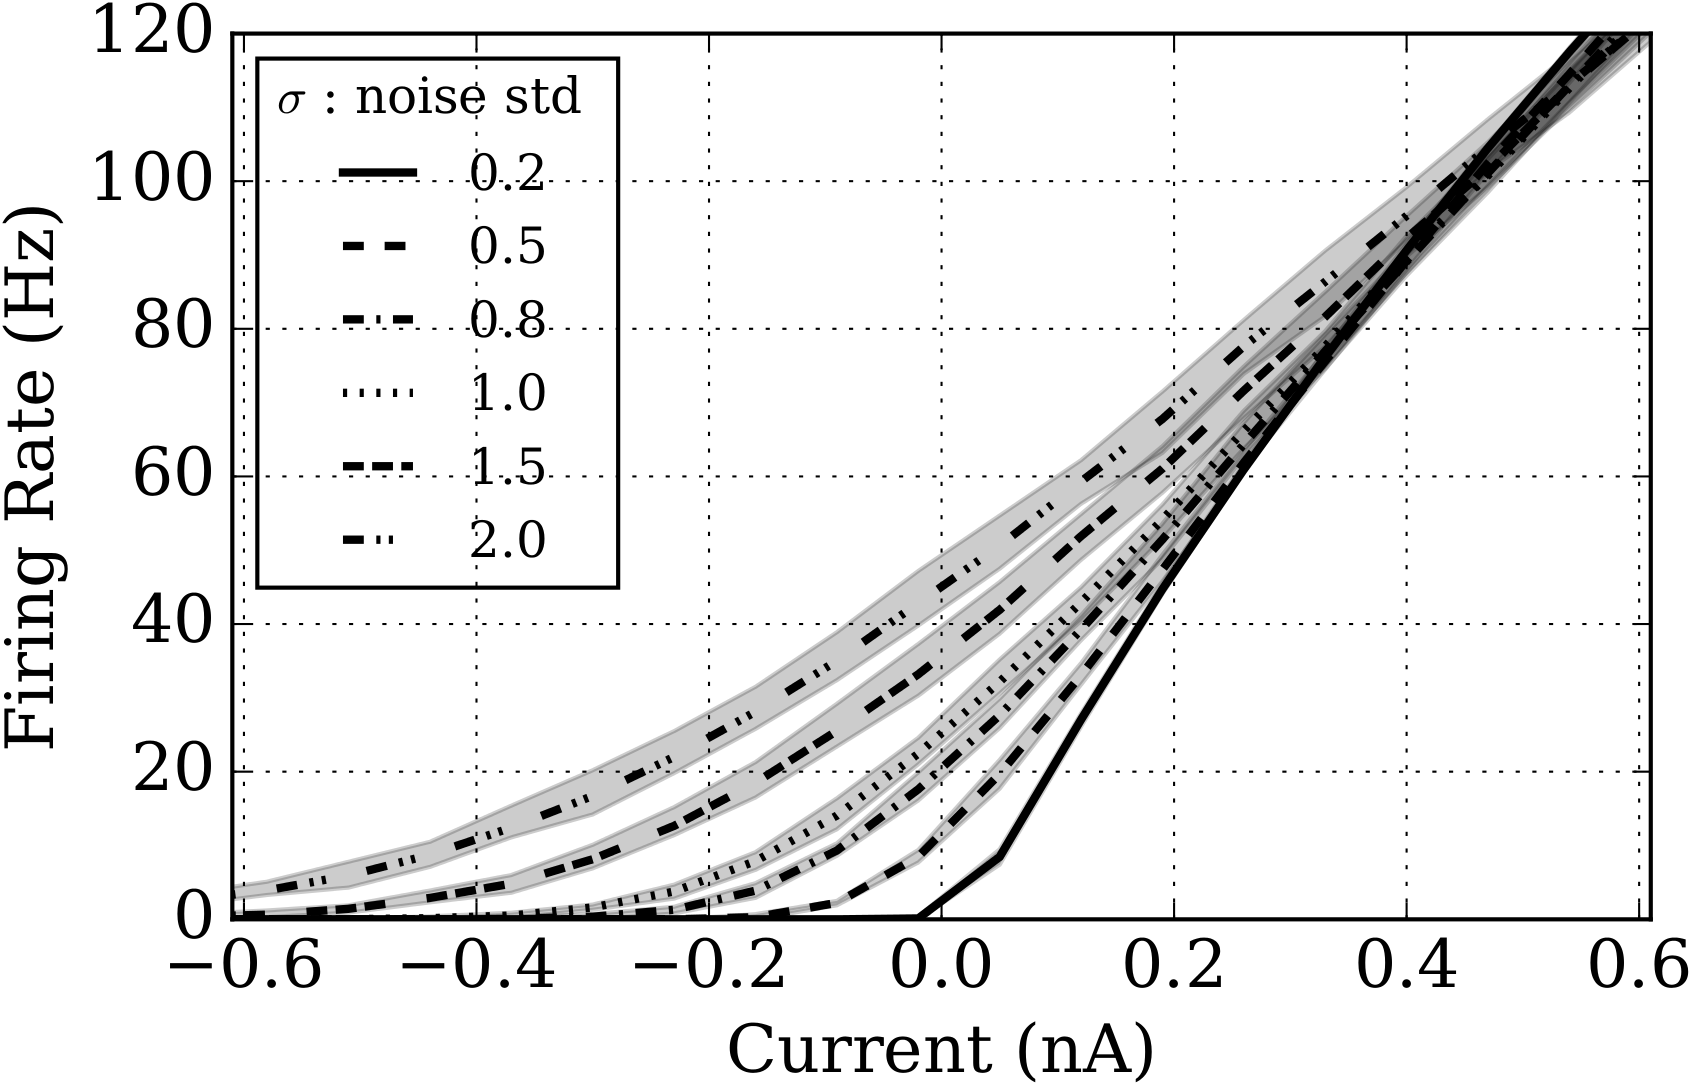
\includegraphics[width=\textwidth]{pics_iconip/siegert.png}
			\caption{Response firing rate of an LIF neuron}
		\end{subfigure}\\
		\begin{subfigure}[t]{0.4\textwidth}
			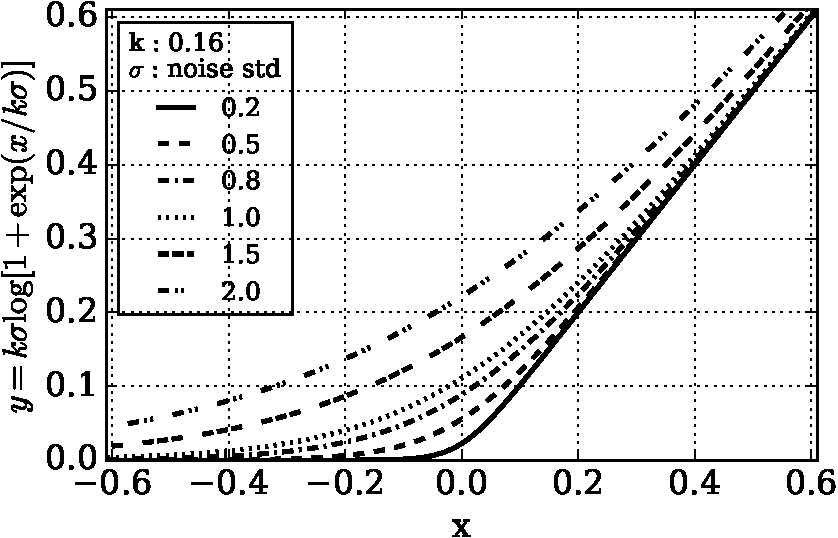
\includegraphics[width=\textwidth]{pics_iconip/4.pdf}
			\caption{NSP}
		\end{subfigure}
		\caption{
			%		NSP fits to the response function of the LIF neuron.
			NSP models the LIF response function.
			(a) Firing rates measured by simulations on an LIF neuron driven by different input currents and discrete noise levels.
			Bold lines show the average and the grey colour fills the range between the minimum and the maximum.
			(b) NSP activates the input $x$ according to different noise levels where $k=0.16$.}
		\label{fig:ns}
	\end{figure}
	To model the response function of LIF neurons (see Figure~\ref{fig:ns}(a)) whose output firing rates are determined by the mean and variance of the noisy input currents, the NSP was proposed:
	\begin{equation}
	y = f_{ns}(x, \sigma) = k \sigma \log [1 + \exp(\frac{x}{k \sigma})]~,
	\label{equ:nsp}
	\end{equation}
	where $x$ and $\sigma$ refer to the mean and standard deviation of the input current, $y$ indicates the intensity of the output firing rate, and $k$, determined by the biological configurations on the LIF neurons~\cite{liu2016noisy}~(listed in Table~\ref{tbl:pynnConfig}), controls the shape of the curves.
	Note that the novel activation function contains two parameters, the mean current and its noise, which can be estimated by:
	\begin{equation}
	x = \tau_{\textit{\textrm{syn}}}\sum_i w_i\lambda_{i}~, ~\sigma^2=\frac{1}{2}\tau_{\textit{\textrm{syn}}}\sum_i w_i^2\lambda_{i}~,
	\label{equ:distr}
	\end{equation}
	where $\lambda_i$ indicates the firing rate of an input spike train.
	%; both are naturally obtained in spiking neurons.
	% With doubled information, more powerful training methods and network models are expected. 
	Figure~\ref{fig:ns}(b) shows the activation function in curve sets corresponding to different discrete noise levels which mimic the responding activities of LIF neurons.
	The derivative of the NSP is the logistic function scaled by $k\sigma$:
	\begin{equation}
	\frac{\partial f_{ns}(x,\sigma)}{\partial x} = \frac{1}{1+exp(-\frac{x}{k\sigma})}~~,
	\label{equ:logist}
	\end{equation}	
	which could be applied easily to back propagation in any ANN training.
	
	\begin{table}[thb]
		\centering
		\caption{\label{tbl:pynnConfig}Default parameter settings for the current-based LIF neurons used through this paper, for PyNN~\cite{davison2008pynn} simulations.}
		\bgroup
		\def\arraystretch{1.4}
		\begin{tabular}{c c c c c c c}
			%\hline
			cm & tau\_m & tau\_refrac & v\_reset & v\_rest& v\_thresh & i\_offset \\
			\hline
			0.25 nF & 20.0 ms & 1.0 ms & -65.0 mV & -65.0 mV & -50.0 mV &  0.1 nA 
		\end{tabular}
		\egroup
	\end{table}
	
	
	\section{Methods}	
	\label{sec:meth}
	
	\subsection{Mapping NSP to Concrete Physical Units}
	\label{sec:af_model}
	The inputs of the NSP, $x$ and $\sigma$, are obtained from physical variables as stated in Equation~\ref{equ:distr}, thus they are already in physical units (nA).
	Therefore, linearly scaling up the activation function by a factor~$S$~(Hz~/~nA) can approximate the output firing rate $\lambda_{\textit{\textrm{out}}}$ of an LIF neuron in Hz:
	\begin{equation}
	\lambda_{\textit{\textrm{out}}} \simeq f_{ns}(x, \sigma) \times S = k \sigma \log [1 + \exp(\frac{x}{k \sigma})] \times S~.
	\label{equ:fit}
	\end{equation}	
	
	
	Suitable calibrations of $k$ and $S$ in Equation~\ref{equ:fit} enables NSP to closely match the practical response firing rates of LIF neurons given various biological parameters.
	The parameter pair of $(k, S)$ is curve-fitted with the triple data points of $(\lambda_{\textit{\textrm{out}}}, x, \sigma)$ and the calibration currently is conducted by linear least squares regression.
	The output firing rate $\lambda_{\textit{\textrm{out}}}$ is measured from SNN simulations where an LIF neuron is driven by synaptic input current of Poisson spike trains.
	Figure~\ref{Fig:nsptau1} shows two calibration results in which the parameters were fitted to $(k, S)=(0.19,208.76)$ when the synaptic constant is set to $\tau_{\textit{\textrm{syn}}}=1$~ms and was fitted to $(k, S)=(0.35,201.06)$ when $\tau_{\textit{\textrm{syn}}}=10$~ms.
	%numerical analysis is considered however for future work to express the factors with biological parameters of an LIF neuron.
	
	\begin{figure}
		\centering
		\begin{subfigure}[t]{0.4\textwidth}
			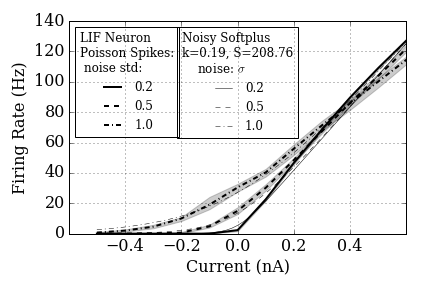
\includegraphics[width=\textwidth]{pics_iconip/4-1.png}
			\caption{$\tau_{\textit{\textrm{syn}}}$=1~ms}
		\end{subfigure}
		\begin{subfigure}[t]{0.4\textwidth}
			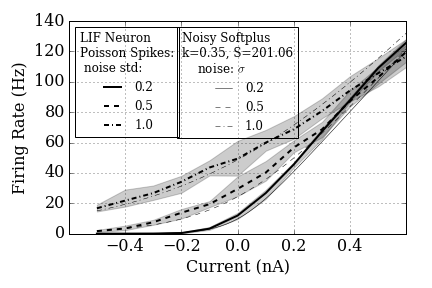
\includegraphics[width=\textwidth]{pics_iconip/4-10.png}
			\caption{$\tau_{\textit{\textrm{syn}}}$=10~ms}
		\end{subfigure}
		\caption{NSP fits to the response firing rates of LIF neurons in concrete physical units.
		Recorded response firing rate of an LIF neuron driven by synaptic current with two synaptic time constants: (a) $\tau_{\textit{\textrm{syn}}}$=1~ms and (b) $\tau_{\textit{\textrm{syn}}}$=10~ms. Averaged firing rates of simulation trails are shown in bold lines, and the grey colour fills the range between the minimum to maximum of the firing rates. The thin lines are the scaled NSP.}
		\label{Fig:nsptau1}
	\end{figure}
	
	\subsection{Parametric Activation Functions~(PAFs)}
	\begin{figure}[tbh!]
		\centering
		\begin{subfigure}[t]{0.49\textwidth}
			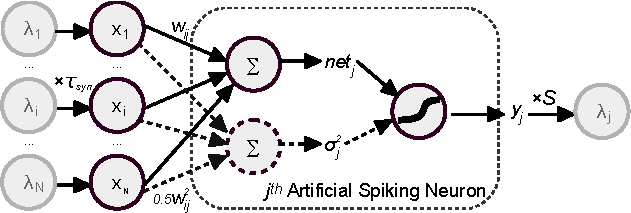
\includegraphics[width=\textwidth]{pics_iconip/neuron_o.pdf}
			\caption{An artificial spiking neuron modelled by NSP.}
		\end{subfigure}\\
		\begin{subfigure}[t]{0.42\textwidth}
			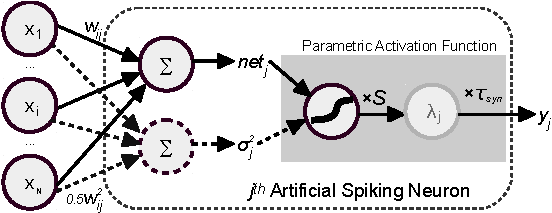
\includegraphics[width=\textwidth]{pics_iconip/neuron_PAF.pdf}
			\caption{An artificial spiking neuron modelled by PAF-NSP.}
		\end{subfigure}
		\caption{The PAF links the firing activity of a spiking neuron to the numerical value of ANNs.}
		\label{Fig:tneuron}
	\end{figure}
	
	
	Neurons in ANNs take inputs from their previous layer, and feed the weighted sum of their input, $net_j = \sum_i w_{ij}x_i$, to the activation function.
	The transformed signal then forms the output of an artificial neuron, which can be denoted as $y_j=f(net_j)$, see Figure~\ref{Fig:compare_as}(a).
	However, a spiking neuron modelled by NSP takes the firing rate as its input/output, thus Equation~\ref{equ:distr} can be written as:
	\begin{equation}
	net_j = \sum_i w_{ij}(\lambda_{i}\tau_{\textit{\textrm{syn}}})~,
	~\sigma^2_j= \sum_i (\frac{1}{2} w_{ij}^2)(\lambda_{i}\tau_{\textit{\textrm{syn}}})~, 
	% \textrm{~~and~~} x_i = \lambda_{i}\tau_{\textit{\textrm{syn}}}~.
	\label{equ:mi_input}
	\end{equation}
	and input $ x_i $ of an artificial neuron can be seen as $x_i=\lambda_{i}\tau_{\textit{\textrm{syn}}}$, see Figure~\ref{Fig:tneuron}(a).
	

	If instead of multiplying every input by $\tau_{\textit{\textrm{syn}}}$ [left of Fig.~\ref{Fig:tneuron}(a)] we do it in every output after $\lambda_j$, [right of Fig.~\ref{Fig:tneuron}(b)] we obtain the same neuron model and structure as a typical neuron in ANNs, See Figure~\ref{Fig:compare_as}(a), that neurons take $x$ as input and output $y$.
%	The PAF version of the activation function (Eq.~\ref{equ:PAF}) will be linearly-scaled by the conversion parameter $S$ and the synaptic time constant $\tau_{syn}$:
	The only difference lies in the activation function where the artificial spiking neuron takes PAF, which is a simple linearly-scaled activation function with a parameter $p$, which is determined by the product of the scaling parameter $S$ and the synaptic time constant $\tau_{\textit{\textrm{syn}}}$:

\begin{equation}
	y = p \times f(x) = S \times \tau_{\textit{\textrm{syn}}} \times f(x)~,
	\label{equ:PAF}
	\end{equation}
	and its derivative function, which is used for back propagation, is:
	\begin{equation}
	\frac{\partial y}{\partial x} = p \times f'(x) = S \times \tau_{\textit{\textrm{syn}}} \times f'(x)~.
	\end{equation}
	
	Excitingly, PAF not only allows NSP to model spiking LIF neurons on ANNs, once the parameter $p$ is acquired the PAF can be generalised to other activation functions.
	Note that the calculation of noise level is not necessary for other activation functions, for example, it can be set to a constant for Softplus or 0 for ReLU.
	%\begin{figure}[bh!]
	%	\centering
	%	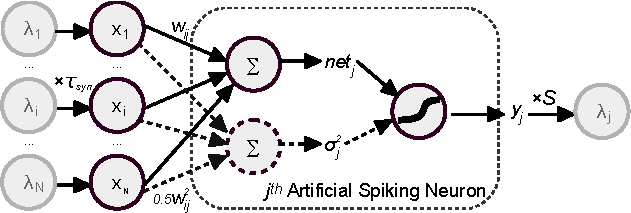
\includegraphics[width=0.8\textwidth]{pics_iconip/neuron_o.pdf}
	%	\caption{Artificial spiking neuron takes scaled firing rates as input, then transforms weighted sum in some activation unit to its output which can be scaled-up to the firing rate of an output spike train.}
	%	\label{Fig:sneuron}
	%\end{figure}
	%
	%NSP transforms the noisy current with parameters of $(net_j, \sigma_j)$ to the equivalent ANN output $y_j$ , where it can be scaled up by the factor $S$ to the firing rate of SNNs.
	%Note that the calculation of noise level is not necessary for activation functions other than NSP, for example, it can be set to a constant for Softplus or 0 for ReLU.
	%We name the neuron model `artificial spiking neurons' which takes firing rates of spike trains as input and output. 
	%The entire artificial spiking neuron model is then generalised to any ReLU/Softplus-like activation functions, See Figure~\ref{Fig:sneuron}.
	%
	%
	%
	%%	Figure~\ref{Fig:sneuron} shows an complete transformation process of a spiking neuron, which mimics the biological neurons taking and generating spike trains.
	%Referred to Figure~\ref{Fig:sneuron}, if we move the left end process of $\times \tau_{\textit{\textrm{syn}}}$ to the right end after $\lambda_j$, Figure~\ref{Fig:sneuron} forms the same neuron model and structure as multilayer perceptron: neurons take $x$ as input and outputs $y$, and this conversion is illustrated in Figure~\ref{Fig:tneuron}.
	%The process within such an artificial neuron is divided into weighted summation and activation, which also applies to SNN modelling by combining the scaling factor $S$ and the synaptic time constant $\tau_{\textit{\textrm{syn}}}$ to activation functions.
	%Thus the combined activation function for modelling SNNs should be:
	%\begin{equation}
	%y = f(x) \times S \times \tau_{\textit{\textrm{syn}}}~~,
	%\label{equ:full_act}
	%\end{equation}
	%and its derivative function which is used when back propagates is:
	%\begin{equation}
	%\frac{\partial y}{\partial x} = f'(x) \times S \times \tau_{\textit{\textrm{syn}}}~~.
	%\end{equation}
	%
	%\begin{figure}[tbh!]
	%	\centering
	%	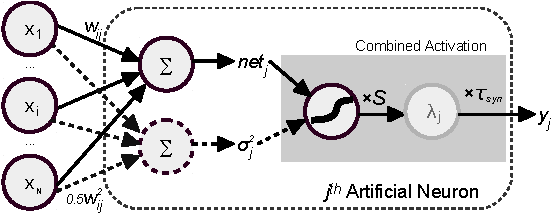
\includegraphics[width=0.8\textwidth]{pics_iconip/neuron_t.pdf}
	%	\caption{Transforming artificial spiking neurons to artificial neurons for SNN modelling. The combined activation links the firing activity of a spiking neuron to the numerical value of ANNs.}
	%	\label{Fig:tneuron}
	%\end{figure}
	
	\subsection{Generalised SNN Training}
	\label{subsec:ns_train}

	The simple change on activation functions presented in the previous section allows the use of common ANN training methods to obtain SNN-compatible weights.
	Consequently, training SNNs can be done in three simple steps: 
	\begin{enumerate}
		\item Calibrate the parameters $(k, S)$ for Noisy Softplus which models response firing rates of LIF neurons, thus to estimate parameter $p=S \times \tau_{\textit{\textrm{syn}}}$ for PAFs. Since $(k, S)$ are solely dependent on the biological configurations of an LIF neuron, the same $p$ can be used for different activation functions and network architectures.
		\item Train any feed-forward ANN with a PAF version of an activation function.
		Training compatibility allows us to choose computationally simple activation functions to increase training speed.
%		Surprisingly, the use of PAF-ReLU provides the best accuracy scores for an SNN on the MNIST dataset. 
		\item Transfer the weights directly to the SNN, which should use the same LIF characteristics used in Step 1.
	\end{enumerate}

	%Thus, once the parameters are tuned for a certain LIF configuration, they can be used for trainings with various activation functions.
	
	%todo
%	This generalised SNN training allows the use of widely-used activation functions in ANNs which are of low complexity and their corresponding derivative functions can be directly used for back propagation.
%	Especially, ReLU, the simplest and most effective activation function may improve the training performance of SNNs.
%	Ideally, the method can be applied for any feedforward network using ReLU-like activation functions, including deep architectures.
%	Most significantly, the ANN-trained weights are ready for use to transfer to SNNs without any conversion, and the output firing rate of a spiking neuron can be obtained in the ANN simulation thus to estimate the power use in Neuromorphic systems (hardware SNN simulators).
	
	
	
	\subsection{Fine Tuning}
	We can train the network with any PAF as stated above, and then fine-tune it with PAF-NSP in the hope of improving the performance of the equivalent SNN by closely modelling the spiking neurons with NSP.
%	both the learning performance provided by ReLU and practical network activities of SNNs modelled by NSP.
	Additionally, we add a small number, for example 0.01, to all the binary values of the labels on the training data.
	Although binary labels enlarges the disparities between the correct recognition label and the rest for better classification capability, 
	spiking neurons seldom stay silent even with negative current influx, thus setting labels to 0 are not practical for training SNNs.
	Therefore, adding an offset relaxes the strict objective function of predicting exact labels with binary values.
%	Instead, it allows a small offset to the objective.
%	An alternative method is to use Softmax function at the top layer, which aims to map real vectors to the range $(0,1)$ that add up to 1. 
%	However, without a limit on the input of Softmax, it will be easy to reach or even exceed the highest firing rate of a spiking neuron.

	
	There are two aspects to the fine tuning which make the ANN closer to SNNs:
	Firstly, using the NSP activation functions causes every single neuron to run as a similar noise level as in SNNs, thus the weights trained by other activation functions will be tuned to fit closer to SNNs.
	Secondly, the output firing rate of any LIF neuron is greater than zero as long as noise exists in their synaptic input.
	Thus adding up a small offset on the labels directs the model to approximate practical SNNs. 
	The result of fine tuning on a Convnet will be demonstrated in Section~\ref{subsec:result_compare}.
	
	\section{Results}
	\label{sec:result}
	
	\subsection{Experiment Description}
	% Architecture
	A spiking ConvNet was trained on MNIST~\cite{lecun1998gradient} dataset, 
	%a popular database in neuromorphic vision, 
	using the generalised SNN training method stated above.
	The architecture (784-6c-6p-12c-12p-10fc) contains $28\times28$ input units, followed by two convolution-pooling layers with 6 and 12 convolutional kernels each, and 10 output neurons fully connected to the last pooling layer to represent the classified digit.
	
	% Training
	To train the ConvNet, firstly, we estimated parameter $p$ for PAFs given LIF configurations listed in Talbe~\ref{tbl:pynnConfig} and $\tau_{\textit{\textrm{syn}}}=5$~ms, $p = S \times \tau_{\textit{\textrm{syn}}} = 1.005$, where $(k=0.30, S=201)$ were calibrated using NSP. 
	Secondly, the training employed PAFs with three core activation functions: ReLU, Softplus and NSP to compare their learning and recognition performance.
%	The parameter $p$ was estimated as $p = S \times \tau_{\textit{\textrm{syn}}} = 1.005$ by calibrating the NSP with LIF response firing rate: $(k=0.30, S=201)$ given $\tau_{\textit{\textrm{syn}}}=5 ms$.
%	The pixel intensities of the input images were normalised to 100~Hz to represent the firing rates of the input spikes.
	The weights were updated using a decaying learning rate, 50 images per batch and 20 epochs.
	Finally, the trained weights were then directly transferred to the corresponding spiking ConvNets for recognition test on the SNN simulator, NEST~\cite{gewaltig2007nest}.
	To validate the effect of fine tuning, we took another training epoch to train these models with PAF-NSP with data labels shifted by $+0.01$.
	Then the weights were also tested on SNN simulations to compare with the ones before fine-tuning.
	
%	The recognition test took the whole testing dataset of MNIST which contains $10,000$ images.
	At the testing stage, the input images were converted to Poisson spike trains~\cite{liu2016bench} and presented for 1~s each.
	The output neuron which fired the most indicated the classification of an input image.

%	The LIF neurons had the same parameters as in training.

%	Moreover, a `fine tuning' test took the trained model for fine tuning, and the tuned weights were tested on the same SNN environment.
%	The tuning only ran for one epoch, 5\% of the cost of the ANN training (20~epochs), using NSP neurons with labels shifted by $+0.01$.
	
	\subsection{Neural Activity}
	\label{subsec:activity}
	To validate how well the NSP activation fits to the response firing rate of LIF neurons in SNNs, we simulated one of the PAF-NSP trained ConvNets on NEST.
%	A small test consisted of ten MNIST digits presented as Poisson spike trains for 1~s each.
	Ten testing images were convolved with a trained $5\times5$ kernel, and the output firing rates of the spiking neurons were recorded and compared to the predictions of these PAFs: $\lambda' = S \times f(x) = y/\tau_{\textit{\textrm{syn}}}$.
	%The input $x$ of the network was calculated as Equation~\ref{equ:mi_input}: $x_i=\lambda_i\tau_{\textit{\textrm{syn}}}$, and so as the weighted sum of the synaptic current (see Equation~\ref{equ:mi_input}), $net_j$ and its variance (see Equation~\ref{equ:si_input}), $\sigma^2_j$.
	%With three combined activation functions as Equation~\ref{equ:full_act}:
	%\begin{equation}
	%\begin{aligned}
	%&\textrm{(1) NSP:~~}  y_j=k \sigma_j \log [1 + \exp(\frac{net_j}{k \sigma_j})] \times S \times \tau_{\textit{\textrm{syn}}}~~,  \\
	%&\textrm{(2) ReLU:~~ } y_j=max(0, net_j) \times S \times \tau_{\textit{\textrm{syn}}}~~, \\
	%&\textrm{(3) Softplus:~~ } y_j=k \sigma \log [1 + \exp(\frac{net_j}{k \sigma})] \times S \times \tau_{\textit{\textrm{syn}}}~~, ~~~\sigma=0.45,  
	%\end{aligned}
	%\end{equation}	
%	With three PAFs of ReLU, Softplus and NSP, we compare the output to the recorded SNN simulations.
	%ReLU assumes a non-noise current, and Softplus takes a static noise level thus $\sigma_j$ is not used for either of them, meanwhile NSP adapts to noise automatically with $\sigma_j$.
%	The experiment took the sequence of 10 digits to the same kernel and 
	The estimated spike counts using NSP fitted the real recorded firing rate much more accurately than ReLU and Softplus, see Figure~\ref{fig:af_compare}.
	%	Figure~\ref{fig:af_stast} illustrated the statistics of error between the estimation and the recorded firing rate, $err = y_j - \lambda_j$ which formed normal distributions where NSP hold the weakest mean (low in abstract) and lowest standard deviation.
	The Euclidean distance, $\sqrt{\sum_{j}(\lambda_j' - \lambda_j)^2}$, between the spike counts and the predicted firing rates by NSP, ReLU and Softplus was 184.57, 361.64 and 1102.76 respectively.
	We manually selected a static noise level of 0.45 for Softplus, whose estimated firing rates located roughly on the top slope of the real response activity.
	This resulted in a longer Euclidean distance than using ReLU, since most of the input noisy currents were of relatively low noise level in this experiment.
	Hence, the firing rate driven by the lower noise level is closer to ReLU curve than Softplus.
	
	\begin{figure}[hb!]
		\centering
		\begin{subfigure}[hb]{0.32\textwidth}
			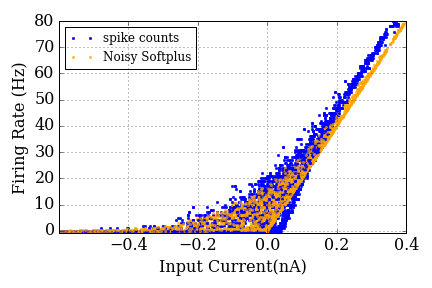
\includegraphics[width=\textwidth]{pics_iconip/6-5-3.png}
			\caption{NSP}
		\end{subfigure}
		\begin{subfigure}[hb]{0.32\textwidth}
			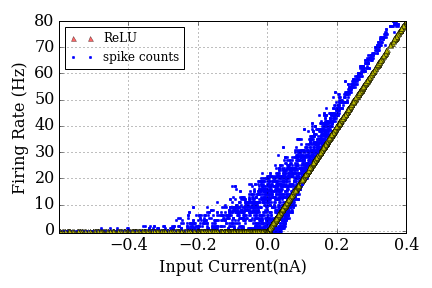
\includegraphics[width=\textwidth]{pics_iconip/6-5-2.png}
			\caption{ReLU}
		\end{subfigure}
		\begin{subfigure}[hb]{0.32\textwidth}
			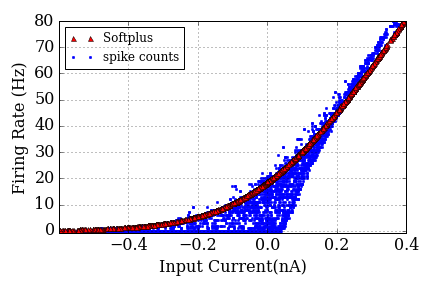
\includegraphics[width=\textwidth]{pics_iconip/6-5-1.png}
			\caption{Softplus}
		\end{subfigure}
		\caption{
			The recorded firing rate of the convolution of the same kernel with 10 images in SNN simulation, compared to the firing rate prediction by $S \times f(x)$.
			NSP (a) fits to the neural response firing rate of LIF neurons more closely than ReLU (b) and Softplus (c).}
		\label{fig:af_compare}
	\end{figure}		
	
%	The SNN successfully classified the digits where the correct label neuron fired the most.
%	We trained the network with binary labels on the output layer, thus the expected firing rate of correct classification was $1/\tau_{\textit{\textrm{syn}}}=200$~Hz according to Equation~\ref{Fig:tneuron}.
%	The firing rates of the recognition test fell to the valid range around 0 to 200~Hz.
	This shows another advantage of the NSP that we can estimate the firing rate of an SNN by $S \times f_{\textit{\textrm{NSP}}}(x)$ running its equivalent ANN, instead of simulating SNNs.
	Moreover, we can constrain the expected firing rate of the top layer, thus preventing the SNN from exceeding its maximum firing rate, for example 1~KHz when the time resolution of the simulation is set to 1~ms.
	
	
	\subsection{Learning Performance}
	%Here we focus on the recognition performance of the proposed ANN-trained SNN method.
	Before looking into the recognition results, it is significant to see the learning capability of the novel activation function, NSP.
	We compared the training using ReLU, Softplus, and NSP by their loss during training averaged over three trials, see Figure~\ref{Fig:loss_ns}.
	ReLU learned fastest with the lowest loss, thanks to its steepest derivative.
	In comparison, Softplus accumulated spontaneous `firing rates' layer-by-layer and its derivative may experience gradual or even vanishing gradients during back propagation, which result in a more difficult training.
	The performance of NSP lied between these two in terms of loss and learning speed.
	The loss stabilised to the same level of the Softplus', because of the same problem of gradual gradients.
	However, it stabilised faster thanks to the accurate modelling of the noise, which means a possibly shorter training time.
	%\begin{figure}[tbp!]
	%	\centering
	%	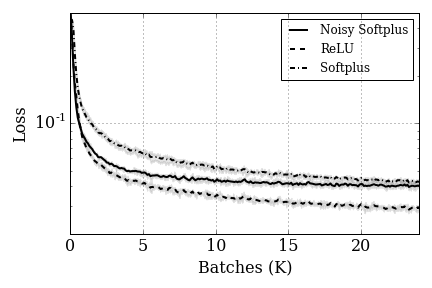
\includegraphics[width=0.7\textwidth]{pics_iconip/8.png}
	%	\caption{Comparisons of Loss during training using NSP, ReLU and Softplus activation functions. Bold lines show the average of three training trials, and the grey colour illustrates the range between the minimum and the maximum values of the trials.  }
	%	\label{Fig:loss_ns}
	%\end{figure}
	%	The trained networks were scaled to SNNs and compared on recognition rates, 93.34\%, 96.43\% and 97.03\% with a conversion loss of 4.76\%, 0.91\% and 0.74\%.
	
	
	\begin{figure}[hb!]
			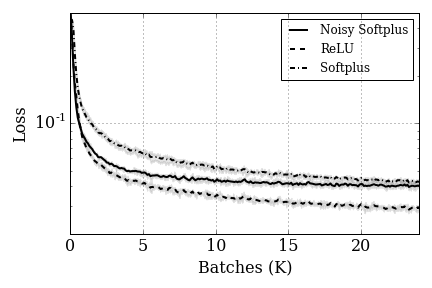
\includegraphics[width=0.4\textwidth]{pics_iconip/8.png}
			\caption{Comparisons of Loss during training using PAF version of NSP, ReLU and Softplus. Bold lines show the average of three training trials, and the grey colour illustrates the range between the minimum and the maximum values of the trials.}
			\label{Fig:loss_ns}
	\end{figure}
	\begin{figure}[hb]
			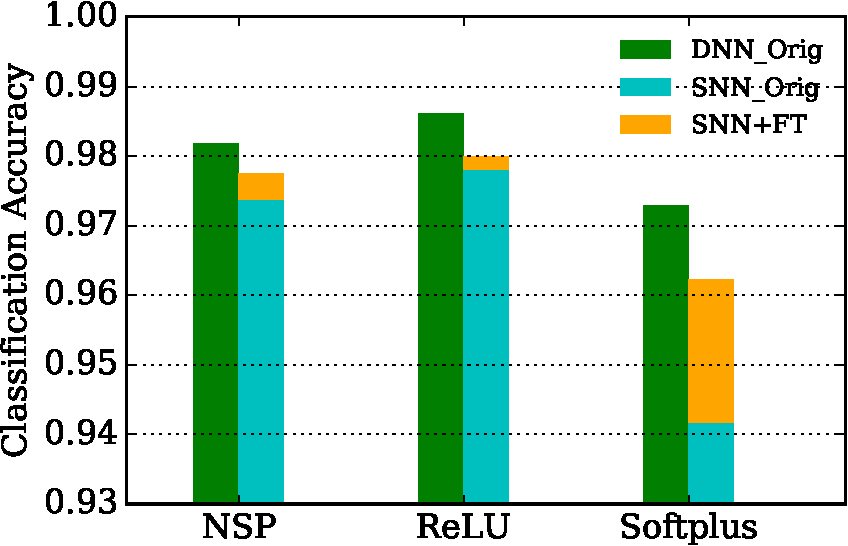
\includegraphics[width=0.4\textwidth]{pics_iconip/9-2.pdf}
			\caption{Classification accuracy.
			The trained weights were tested using the same activation function as training (DNN\_Orig), then transferred to SNN and tested on NEST simulation (SNN\_Orig), and finally fine-tuned to be tested on SNN (SNN\_FT) as well.  }
			\label{Fig:result_bar}
	\end{figure}


	
	
	
	
	\subsection{Recognition Performance}
	\label{subsec:result_compare}
	The classification errors for the tests are investigated by comparing the average classification accuracy among three trials, shown in Figure~\ref{Fig:result_bar}.
	At first, all trained models were tested on the same artificial neurons as used for training in ANNs, and these experiments were called the `DNN' test since the network had a deep structure (6 layers).
	Subsequently, the trained weights were directly applied to the SNN without any transformation, and these `SNN' experiments tested their recognition performance on the NEST simulator.
	From DNN to SNN, the classification accuracy declines by 0.80\%, 0.79\% and 3.12\% on average for NSP, ReLU and Softplus.
	The accuracy loss was caused by the mismatch between the activations and the practical response firing rates, see examples in Figure~\ref{fig:af_compare}, and the strict binary labels for NSP and Softplus activations.
	Fortunately, the problem is alleviated by fine tuning which increased the classification accuracy by 0.38\%, 0.19\% and 2.06\%, and resulted in the total loss of 0.43\%, 0.61\%, and 1.06\% respectively.
%	The order of total losses of these activation functions followed the Euclidean distance measured in Section~\ref{subsec:activity}.
	Softplus benefits the most from fine tuning, since the huge mismatch~(Figure~\ref{fig:af_compare}(c)) of response firing rate is greatly corrected.
	The improvement of NSP was obtained from the offset on the labels which helps the network to fit practical SNNs.
	As the recognition performance of ReLU is already high, there's little room for improvement.
	Even though the fine-tuning procedure does its job, the gain in accuracy is the smallest for this activation function.
	
	%	Thus fine tuning mainly corrects the mismatch between ReLU and the firing rates in SNNs, and constraints the output firing rates of the network.
	
  %	Thus fine tuning mainly corrects the mismatch between ReLU and the firing rates in SNNs, and constraints the output firing rates of the network.
%	Softplus benefits the most from fine tuning, since not only the huge mismatch of response firing rate is greatly corrected, but also the offset on the labels helps the network to fit SNNs. 
	%dummy change

	%\begin{figure}[hbt!]
	%	\centering
	%	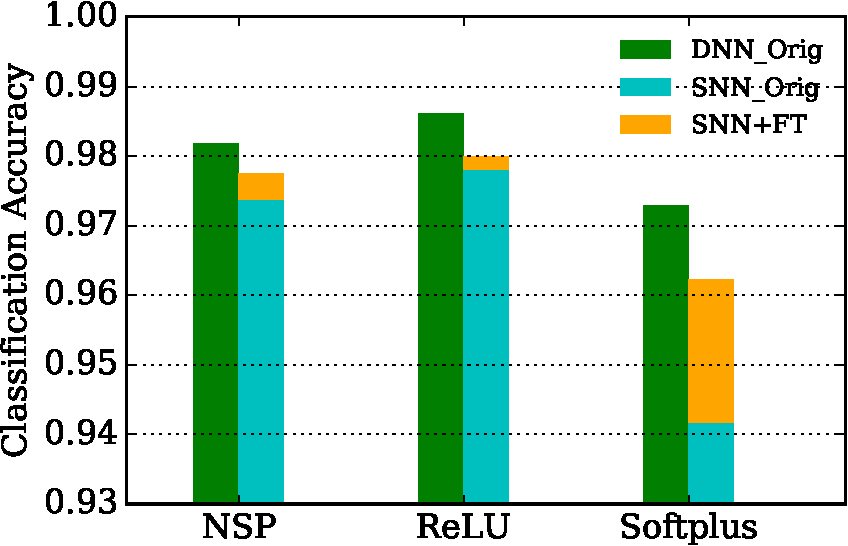
\includegraphics[width=0.7\textwidth]{pics_iconip/9-2.pdf}
	%	\caption{Classification accuracy compared among trained weights of NSP, ReLU, Softplus on DNN, SNN and fine-tuned SNN.}
	%	\label{Fig:result_bar1}
	%\end{figure}
	
	%\begin{table}[tbh] 
	%	\caption{Comparisons of classification accuracy (in \%) of ANN-trained convolutional neural models on original DNN, NEST simulated SNN, and SNN with fine-tuned (FT) model.}
	%	\begin{center}
	%		\bgroup
	%		\def\arraystretch{1.5}
	%		\begin{tabular} {r |c  c c |c c c |c c c}
	%			%First line
	%			\hline
	%			Trial No.
	%			&\multicolumn{3}{c|}{1} 
	%			&\multicolumn{3}{c|}{2}
	%			&\multicolumn{3}{c}{3}\\
	%			\hline
	%			Model
	%			& DNN & SNN &FT
	%			& DNN & SNN &FT
	%			& DNN & SNN &FT\\
	%			\hline
	%			\textbf{Noisy Sofplus}
	%			& 1.91 & 2.76 &2.45
	%			& 1.79 & 2.56 &2.19
	%			& 1.76 & 2.55 &2.10\\
	%			%				& 98.09 & 97.24 &97.55
	%			%				& 98.21 & 97.44 &97.81
	%			%				& 98.24 & 97.45 &97.90\\
	%			%				\hline
	%			\textbf{ReLU}
	%			& 1.36 & 2.03 &1.88
	%			& 1.46 & 2.28 &2.00
	%			& 1.36 & 2.25 &2.12\\
	%			%				& 98.64 & 97.97 &98.12
	%			%				& 98.54 & 97.72 &98.00
	%			%				& 98.64 & 97.75 &97.88\\
	%			%				\hline
	%			\textbf{Sofplus}
	%			& 2.30 & 5.66 &3.91
	%			& 2.75 & 5.22 &3.55
	%			& 2.42 & 6.62 &3.87\\
	%			%				& 97.70 & 94.34 &96.09
	%			%				& 97.25 & 94.78 &96.45
	%			%				& 97.58 & 93.38 &96.13\\
	%			\hline
	%		\end{tabular}
	%		\egroup
	%		\label{tbl:ns_result}
	%	\end{center}
	%\end{table}
	
	
	
	
	%	The best classification accuracy achieved by SNNs was trained with ReLU and fine-tuned by NSP.
	The most efficient training in terms of both classification accuracy and algorithm complexity, takes PAF-ReLU for ANN training and PAF-NSP for fine tuning.
%	Softplus does not exhibit better classification capability and, more importantly, the manually selected static noise level hugely influences the mismatch between the predicted firing rates and the real data.
%	Although NSP shows the least classification drop from ANNs to SNNs, the training performance is still worse than ReLU.
	%	Improved back propagation or other learning algorithms using noise level will be listed in the future work. 
	The best classification accuracy achieved by a larger spiking ConvNet~(784-16c-16p-64c-64c-10fc) was 98.85\% after fine tuning, a 0.20\% drop from the ANN test (99.05\%).
	The network reached the recognition rate of 98.7\% even without fine tuning, thus we suggest to make fine tuning an optional step for training.
%	which was trained with PAF-ReLU and fine-tuned using PAF-NSP.

	
	It is useful to compare with existing SNN training methods shown in Table~\ref{tbl:compare} where we order them on the computation complexity (descending).
%	The generalised training method this paper proposed wins the other methods over the simplest activation function, and no conversions are requited of trained weights to be transferred to SNNs, they are well fitted to biologically-plausible LIF neurons, and only an optional additive processing of fine tuning.
	The generalised training method presented in this paper has a simple activation function, it requires no conversions of trained weights, which are well fitted to biologically-plausible LIF neurons, and has a single \emph{optional} additional processing of fine tuning.
	The combination of these features compose a method with exceptional performance and ease of use for training SNNs.
	
	
  \begin{table*}[thb!]
	\caption{SNN training methods comparison.}
	\begin{center}
		\bgroup
		\def\arraystretch{1.1}
		\begin{tabular}{l c c c c c c}
			\cline{1-6}
			\begin{mycell}{1cm} Method \end{mycell} & 
			%  					\begin{mycell}{1.8cm} Computation\\Complexity \end{mycell} & 
			\begin{mycell}{1.8cm}Activation\\Function\end{mycell} &
			\begin{mycell}{1.8cm} Biologically-\\plausibility \end{mycell} &  
			\begin{mycell}{1.8cm} Additional\\Processing \end{mycell} &
			\begin{mycell}{1.8cm} Conversion \end{mycell} & 
			\begin{mycell}{1.8cm} Classification\\Accuracy(\%) \end{mycell} 
			\\
			\hline
			\begin{mycell}{1cm} \cite{Jug_etal_2012} \end{mycell} & 
			%  					\begin{mycell}{1.8cm} 1st \end{mycell} & 
			\begin{mycell}{1.8cm}Siegert \end{mycell} &
			\begin{mycell}{1.8cm} \textbf{Yes} \end{mycell} &  
			\begin{mycell}{1.8cm} \textbf{No} \end{mycell} & 
			\begin{mycell}{1.8cm} \textbf{No} \end{mycell} & 
			\begin{mycell}{1.8cm} 94.94~\cite{Stromatias2015scalable} \end{mycell} 
			\\
			\begin{mycell}{1cm} \cite{hunsberger2015spiking} \end{mycell} & 
			%  					\begin{mycell}{1.8cm} 2nd \end{mycell} & 
			\begin{mycell}{1.8cm} Soft LIF \end{mycell} &
			\begin{mycell}{1.8cm} \textbf{Yes} \end{mycell} &  
			\begin{mycell}{2.2cm} Noisy inputs\\ \&Activations \end{mycell} & 
			\begin{mycell}{1.8cm} \textbf{No} \end{mycell} & 
			\begin{mycell}{1.8cm} 98.37 \end{mycell}
			\\
			\begin{mycell}{1cm} \cite{diehl2015fast} \end{mycell} & 
			%  					\begin{mycell}{1.8cm} 3rd \end{mycell} & 
			\begin{mycell}{1.8cm} \textbf{ReLU} \end{mycell} &
			\begin{mycell}{1.8cm} No \end{mycell} &  
			\begin{mycell}{1.8cm} Dropout  \end{mycell} & %\&\\Conversion
			\begin{mycell}{1.8cm} Yes \end{mycell} &  
			\begin{mycell}{1.8cm} \textbf{99.1\%} \end{mycell} 
			\\
			\begin{mycell}{1cm} This\\Paper \end{mycell} & 
			%  					\begin{mycell}{1.8cm} 3rd \end{mycell} & 
			\begin{mycell}{1.8cm} \textbf{PAF}\\($p\times$ReLU)\end{mycell} &
			\begin{mycell}{1.8cm} \textbf{Yes} \end{mycell} &  
			\begin{mycell}{2.2cm} \textbf{No} \\or fine tune  \end{mycell} & 
			\begin{mycell}{1.8cm} \textbf{No} \end{mycell} & 
			\begin{mycell}{2.4cm} 98.70\\ 98.85(fine tune) \end{mycell}  
			\\
			\cline{1-6}
			% contents!
		\end{tabular}
		\egroup
	\end{center}
	\label{tbl:compare}
\end{table*}
	
	%The network structure was the same with the state-of-the-art model which reported the best classification accuracy of 99.1\%~\cite{diehl2015fast} in ANN-trained SNNs: 12c5-2s-64c5-2s-10fc.
	%Their nearly loss-less conversion from ANNs to SNNs was achieved by using IF neurons, while our network performs the best among SNNs consisted of LIF neurons to our knowledge.
	
	\begin{figure}[htb!]
		\centering
		\begin{subfigure}[t]{0.4\textwidth}
			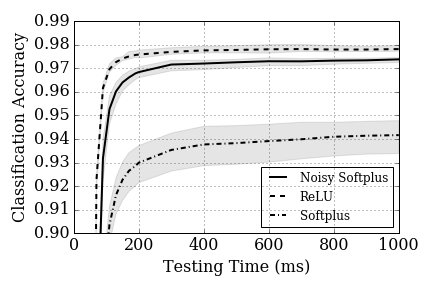
\includegraphics[width=\textwidth]{pics_iconip/8-2.png}
			\caption{Before fine tuning}
		\end{subfigure}
		\begin{subfigure}[t]{0.4\textwidth}
			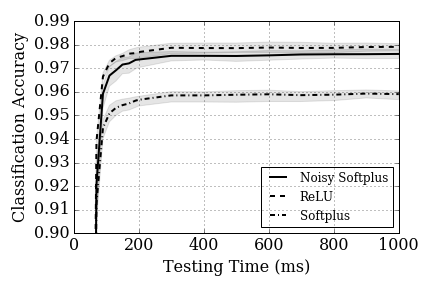
\includegraphics[width=\textwidth]{pics_iconip/8-3.png}
			\caption{After fine tuning.}
		\end{subfigure}
		
		\caption{The classification accuracy of 3 trials (averaged in bold lines, grey shading shows the range between minimum to maximum) over short response times, with (a) trained weights before fine tuning, and (b) after fine tuning.}
		\label{fig:ca_time}	
	\end{figure}
	
	As it is a major concern in neuromorphic vision, the recognition performance over short response times is also estimated in Figure~\ref{fig:ca_time}.
	After fine tuning, Softplus significantly reduced the mismatch since the randomness among the three trials shrinks to a range similar to other experiments.
	Fine tuning also improved its classification accuracy and the response latency.
	Notice that all of the networks trained by three different activation functions showed a very similar stabilisation curve, which means they all reached an accuracy close to their best after only 300~ms of biological time. 
	
	
	\subsection{Power Consumption}
	Neuromorphic engineering aims to build intelligent machines with low power cost~\cite{furber2016large}, thus power consumption is an important metric for evaluating their performance~\cite{liu2016bench}.
	PAF-NSP provides energy estimation for SNNs without running the models on real neuromorphic hardware.
	For a single neuron, the energy consumption of the synaptic events it triggers is:
	\begin{equation}
	E_{j} = \lambda_j' N_j T E_{\textit{\textrm{syn}}} = \dfrac{y_j N_j T E_{\textit{\textrm{syn}}}}{\tau_{\textit{\textrm{syn}}}}~~,
	\label{equ:energy}
	\end{equation}
	where $\lambda_j'$ is the estimated output firing rate, $N_j$ is the number of post-synaptic neurons it connects to, $T$ is the testing time, and $E_{\textit{\textrm{syn}}}$ is the energy cost for a synaptic event of some specific neuromorphic hardware, for example, about 10~nJ on SpiNNaker~\cite{furber2016large}.
	Thus to estimate the whole network, we can sum up all the synaptic events of all the neurons:
	\begin{equation}
	\sum_j E_{j} =  \dfrac{T E_{\textit{\textrm{\textit{\textrm{syn}}}}}}{\tau_{\textit{\textrm{syn}}}} \sum_{j}y_j N_j.
	\end{equation}
	Thus, it may cost SpiNNaker 0.08~W, 240~J running for $3,000$~s with synaptic events of $8\times10^6/$s to classify $10,000$ images (300~ms each) with an accuracy of 98.02\%.
	The best performance reported using the larger network may cost SpiNNaker 0.54~W operating synaptic event rate at $5.34\times10^7/$s, consuming 5340~J to classify all the images for 1~s each.
	
	\section{Conclusion and Future Work}
	We presented a generalised SNN training method to train an equivalent ANN and transfer the trained weights back to SNNs.
	This training procedure consists of two simple stages: first, estimate parameter $p$ for PAF using NSP, and second, use a PAF version of conventional activation functions for ANN training. % can be generalised to activation units other than NSP.
	%The training of a SNN model is exactly the same as ANN training, and 
	The trained weights can be directly used in SNN without any further transformation.
	This method requires the least computation complexity while performing most effectively among existing training algorithms.
	% and even more straight-forward than the other ANN offline training methods which requires an extra step of converting ANN-trained weights to SNN's.
	
	In terms of classification/recognition accuracy, the performance of ANN-trained SNNs is nearly equivalent to ANNs, and the performance loss can be partially solved by fine tuning.
	The best classification accuracy of 98.85\% using LIF neurons in a PyNN simulation outperforms state-of-the-art SNN models of LIF neurons and is very close to the result using IF neurons~\cite{diehl2015fast}.
	An important feature of accurately modelling LIF neurons in ANNs is the acquisition of spiking neuron firing rates. These will aid deployment of SNNs in neuromorphic hardware by providing power and communication estimates, which would allow better usage or customisation of the platforms.
	
	The current limitation prohibiting this off-line SNN training method from wide use lies in the lack of supporting tools, which would enable SNN training on popular deep learning platforms. Additionally an automation tool to read platform-dependent trained weights into the PyNN~\cite{davison2008pynn} language.
	Another issue is the parameter calibration on the scaling factor of the PAF, thus numerical analysis is considered for future work to express the factors with biological parameters of a LIF neuron.
	Interesting applications have started with collaborations on speech recognition of cochlea generated spikes which has achieved a promising accuracy at the initial test-idea stage.
	A further goal is to implement deep networks fit for ImageNet~\cite{deng2009imagenet} tasks on neuromorphic hardware, which will also require modelling various structures of deep learning, for example recurrent neural networks.
	
	\section*{Acknowledgments}
The research leading to these results has received funding from the European Research Council 
(FP/2007-2013) / ERC Grant Agreement n. 320689 and from the EU Flagship Human Brain Project (FP7-604102). 
Yunhua Chen received funding from the Natural Science Foundation of Guangdong Province, China (No: 2016A030313713) and also from  the Natural Science Foundation of Guangdong Province, China (No: 2014A030310169).
%Qian Liu personally thanks to the funding from the National Natural Science Foundation of China (61662013,U1501252), the Guangxi Natural Science Foundation~(2014GXNSFDA118036), and The High Level of Innovation Team of Colleges and Universities in Guangxi and Outstanding Scholars Program Funding.




% if have a single appendix:
%\appendix[Proof of the Zonklar Equations]
% or
%\appendix  % for no appendix heading
% do not use \section anymore after \appendix, only \section*
% is possibly needed

% use appendices with more than one appendix
% then use \section to start each appendix
% you must declare a \section before using any
% \subsection or using \label (\appendices by itself
% starts a section numbered zero.)
%


%\appendices
%\section{Proof of the First Zonklar Equation}
%Appendix one text goes here.

%% you can choose not to have a title for an appendix
%% if you want by leaving the argument blank
%\section{}
%Appendix two text goes here.


% use section* for acknowledgment
\ifCLASSOPTIONcompsoc
  % The Computer Society usually uses the plural form
  \section*{Acknowledgments}
\else
  % regular IEEE prefers the singular form
  \section*{Acknowledgment}
\fi


The authors would like to thank...


% Can use something like this to put references on a page
% by themselves when using endfloat and the captionsoff option.
\ifCLASSOPTIONcaptionsoff
  \newpage
\fi



% trigger a \newpage just before the given reference
% number - used to balance the columns on the last page
% adjust value as needed - may need to be readjusted if
% the document is modified later
%\IEEEtriggeratref{8}
% The "triggered" command can be changed if desired:
%\IEEEtriggercmd{\enlargethispage{-5in}}

% references section

% can use a bibliography generated by BibTeX as a .bbl file
% BibTeX documentation can be easily obtained at:
% http://mirror.ctan.org/biblio/bibtex/contrib/doc/
% The IEEEtran BibTeX style support page is at:
% http://www.michaelshell.org/tex/ieeetran/bibtex/
%\bibliographystyle{IEEEtran}
% argument is your BibTeX string definitions and bibliography database(s)
%\bibliography{IEEEabrv,../bib/paper}
%
% <OR> manually copy in the resultant .bbl file
% set second argument of \begin to the number of references
% (used to reserve space for the reference number labels box)
\bibliographystyle{IEEEtran}
\bibliography{ref}

% biography section
% 
% If you have an EPS/PDF photo (graphicx package needed) extra braces are
% needed around the contents of the optional argument to biography to prevent
% the LaTeX parser from getting confused when it sees the complicated
% \includegraphics command within an optional argument. (You could create
% your own custom macro containing the \includegraphics command to make things
% simpler here.)
%\begin{IEEEbiography}[{\includegraphics[width=1in,height=1.25in,clip,keepaspectratio]{mshell}}]{Michael Shell}
% or if you just want to reserve a space for a photo:

\begin{IEEEbiography}{Qian Liu}
Biography text here.
\end{IEEEbiography}

% if you will not have a photo at all:
\begin{IEEEbiographynophoto}{Yunhua Chen}
Biography text here.
\end{IEEEbiographynophoto}

% insert where needed to balance the two columns on the last page with
% biographies
%\newpage

\begin{IEEEbiographynophoto}{Garibaldi Pineda-Garc\'ia}
Biography text here.
\end{IEEEbiographynophoto}

\begin{IEEEbiographynophoto}{Steve Furber}
Biography text here.
\end{IEEEbiographynophoto}

% You can push biographies down or up by placing
% a \vfill before or after them. The appropriate
% use of \vfill depends on what kind of text is
% on the last page and whether or not the columns
% are being equalized.

%\vfill

% Can be used to pull up biographies so that the bottom of the last one
% is flush with the other column.
%\enlargethispage{-5in}



% that's all folks
\end{document}


